\chapter{The Simplex Method}
\section{Linear Programming and Extreme Points}
In this section we formalize the intuition we've obtained in all our work in two dimensional linear programming problems. Namely, we noted that if an optimal solution existed, then it occurred at an extreme point. For the remainder of this chapter, assume that $A \in \mathbb{R}^{m \times n}$ with full row rank and $b \in \mathbb{R}^m$ let
\begin{equation}
X = \{\mathbf{x} \in \mathbb{R}^n : \mathbf{A}\mathbf{x} \leq \mathbf{b},\;\;\mathbf{x} \geq \mathbf{0}\}
\end{equation}
be a polyhedral set over which we will maximize the objective function $z(x_1,\dots,x_n) = \mathbf{c}^T\mathbf{x}$, where $\mathbf{c},\mathbf{x} \in \mathbb{R}^n$. That is, we will focus on the linear programming problem:
\begin{equation}P\left\{
\begin{aligned}
\max\;\;&\mathbf{c}^T\mathbf{x}\\
s.t.\;\;&\mathbf{A}\mathbf{x} \leq \mathbf{b}\\
& \mathbf{x} \geq \mathbf{0}
\end{aligned}\right.
\end{equation}

\begin{theorem} If Problem $P$ has an optimal solution, then Problem $P$ has an optimal extreme point solution.
\label{thm:EPSoln}
\end{theorem}
\begin{proof} Applying the Cartheodory Characterization theorem, we know that any point $\mathbf{x} \in X$ can be written as:
\begin{equation}
\mathbf{x} = \sum_{i=1}^k\lambda_i\mathbf{x}_i + \sum_{i=1}^l\mu_i\mathbf{d}_i
\end{equation}
where $\mathbf{x}_1,\dots\mathbf{x}_k$ are the extreme  points of $X$ and $\mathbf{d}_1,\dots,\mathbf{d}_l$ are the extreme directions of $X$ and we know that 
\begin{equation}
\begin{aligned}
\sum_{i=1}^{k}\lambda_i & = 1\\
\lambda_i, \mu_i & \geq 0\;\;\forall i
\end{aligned}
\end{equation}
We can rewrite problem $P$ using this characterization as:
\begin{equation}
\begin{aligned}
\max\;\;& \sum_{i=1}^k\lambda_i\mathbf{c}^T\mathbf{x}_i + \sum_{i=1}^l\mu_i\mathbf{c}^T\mathbf{d}_i\\
s.t.\;\; & \sum_{i=1}^{k}\lambda_i = 1\\
&\lambda_i, \mu_i \geq 0\;\;\forall i
\end{aligned}
\end{equation}
If there is some $i$ such that $\mathbf{c}^T\mathbf{d}_i > 0$, then we can simply choose $\mu_i$ as large as we like, making the objective as large as we like, the problem will have no finite solution. 

Therefore, assume that $\mathbf{c}^T\mathbf{d}_i \leq 0$ for all $i=1,\dots,l$ (in which case, we may simply choose $\mu_i = 0$, for all $i$). Since the set of extreme points $\mathbf{x}_1,\dots\mathbf{x}_k$ is finite, we can simply set $\lambda_p = 1$ if $\mathbf{c}^T\mathbf{x}_p$ has the largest value among all possible values of $\mathbf{c}^T\mathbf{x}_i$, $i=1,\dots,k$. This is clearly the solution to the linear programming problem. Since $\mathbf{x}_p$ is an extreme point, we have shown that if $P$ has a solution, it must have an extreme point solution. 
\end{proof}
\begin{corollary} Problem $P$ has a finite solution if and only if $\mathbf{c}^T\mathbf{d}_i \leq 0$ for all $i=1,\dots l$ when $\mathbf{d}_1,\dots,\mathbf{d}_l$ are the extreme directions of $X$.
\label{cor:OptimalityDirections}
\end{corollary}
\begin{proof} This is implicit in the proof of the theorem.
\end{proof}
\begin{corollary} Problem $P$ has alternative optimal solutions if there are at least two extreme points $\mathbf{x}_p$ and $\mathbf{x}_q$ so that $\mathbf{c}^T\mathbf{x}_p = \mathbf{c}^T\mathbf{x}_q$ and so that $\mathbf{x}_p$ is the extreme point solution to the linear programming problem.
\end{corollary}
\begin{proof} Suppose that $\mathbf{x}_p$ is the extreme point solution to $P$ identified in the proof of the theorem. Suppose $\mathbf{x}_q$ is another extreme point solution with $\mathbf{c}^T\mathbf{x}_p = \mathbf{c}^T\mathbf{x}_q$. Then every convex combination of $\mathbf{x}_p$ and $\mathbf{x}_q$ is contained in $X$ (since $X$ is convex). Thus every $\mathbf{x}$ with form $\lambda\mathbf{x}_p + (1-\lambda)\mathbf{x}_q$ and $\lambda \in [0,1]$ has objective function value:
\begin{displaymath}
\lambda\mathbf{c}^T\mathbf{x}_p + (1-\lambda)\mathbf{c}^T\mathbf{x}_q = 
\lambda\mathbf{c}^T\mathbf{x}_p + (1-\lambda)\mathbf{c}^T\mathbf{x}_p = 
\mathbf{c}^T\mathbf{x}_p
\end{displaymath}
which is the optimal objective function value, by assumption.
\end{proof}

\begin{exercise} Let $X = \{\mathbf{x} \in \mathbb{R}^n : \mathbf{A}\mathbf{x} \leq \mathbf{b},\;\;\mathbf{x} \geq \mathbf{0}\}$ and suppose that $\mathbf{d}_1,\dots\mathbf{d}_l$ are the extreme directions of $X$ (assuming it has any). Show that the problem:
\begin{equation}
\begin{aligned}
\min\;\;&\mathbf{c}^T\mathbf{x}\\
s.t.\;\;&\mathbf{A}\mathbf{x} \leq \mathbf{b}\\
& \mathbf{x} \geq \mathbf{0}
\end{aligned}
\end{equation}
has a finite optimal solution if (and only if) $\mathbf{c}^T\mathbf{d}_j \geq 0$ for $k=1,\dots,l$. [Hint: Modify the proof above using the Cartheodory characterization theorem.] 
\label{exer:MinDirections}
\end{exercise}

\section{Algorithmic Characterization of Extreme Points}
In the previous sections we showed that if a linear programming problem has a solution, then it must have an extreme point solution. The challenge now is to identify some simple way of identifying extreme points. To accomplish this, let us now assume that we write $X$ as:
\begin{equation}
X = \{\mathbf{x} \in \mathbb{R}^n : \mathbf{A}\mathbf{x} = \mathbf{b},\;\;\mathbf{x} \geq \mathbf{0}\}
\end{equation}
Our work in the previous sections shows that this is possible. Recall we can separate $\mathbf{A}$ into an $m\times m$ matrix $B$ and an $m \times (n-m)$ matrix $N$ and we have the result:
\begin{equation}
\mathbf{x}_\mathbf{B} = \mathbf{B}^{-1}\mathbf{b} - \mathbf{B}^{-1}\mathbf{N}\mathbf{x}_\mathbf{N}
\label{eqn:BasicVars2}
\end{equation}
We know that $\mathbf{B}$ is invertible since we assumed that $\mathbf{A}$ had full row rank. If we assume that $\mathbf{x}_\mathbf{N} = \mathbf{0}$, then the solution
\begin{equation}
\mathbf{x}_\mathbf{B} = \mathbf{B}^{-1}\mathbf{b}
\end{equation}
was called a \textit{basic solution} (See Definition \ref{def:BasicSoln}.) Clearly any basic solution satisfies the constraints $\mathbf{A}\mathbf{x} = \mathbf{b}$ but it may not satisfy the constraints $\mathbf{x} \geq \mathbf{0}$. 

\begin{definition}[Basic Feasible Solution] If $\mathbf{x}_\mathbf{B} = \mathbf{B}^{-1}\mathbf{b}$ and $\mathbf{x}_\mathbf{N} = \mathbf{0}$ is a basic solution to $\mathbf{A}\mathbf{x} = \mathbf{b}$ and $\mathbf{x}_\mathbf{B} \geq 0$, then the solution $(\mathbf{x}_\mathbf{B},\mathbf{x}_\mathbf{N})$ is called \textit{basic feasible solution}.
\end{definition}

\begin{theorem} Every basic feasible solution is an extreme point of $X$. Likewise, every extreme point is characterized by a basic feasible solution of $\mathbf{A}\mathbf{x} = \mathbf{b}, \mathbf{x} \geq \mathbf{0}$.
\label{thm:BFSEP}
\end{theorem}
\begin{proof} Since $\mathbf{A}\mathbf{x} = \mathbf{B}\mathbf{x}_\mathbf{B} + \mathbf{N}\mathbf{x}_\mathbf{N} = \mathbf{b}$ this represents the intersection of $m$ linearly independent hyperplanes (since the rank of $\mathbf{A}$ is $m$). The fact that $\mathbf{x}_\mathbf{N} = \mathbf{0}$ and $\mathbf{x_N}$ contains $n-m$ variables, then we have $n-m$ binding, linearly independent hyperplanes in $\mathbf{x}_\mathbf{N} \geq 0$. Thus the point $(\mathbf{x}_\mathbf{B}, \mathbf{x}_\mathbf{N})$ is the intersection of $m + (n-m) = n$ linearly independent hyperplanes. By Theorem \ref{thm:DefExtremePoint} we know that $(\mathbf{x}_\mathbf{B}, \mathbf{x}_\mathbf{N})$ must be an extreme point of $X$. 

Conversely, let $\mathbf{x}$ be an extreme point of $X$. Clearly $\mathbf{x}$ is feasible and by Theorem \ref{thm:DefExtremePoint} it must represent the intersection of $n$ hyperplanes. The fact that $\mathbf{x}$ is feasible implies that $\mathbf{A}\mathbf{x} = \mathbf{b}$. This accounts for $m$ of the intersecting linearly independent hyperplanes. The remaining $n-m$ hyperplanes must come from $\mathbf{x} \geq \mathbf{0}$. That is, $n-m$ variables are zero. Let $\mathbf{x}_\mathbf{N} = \mathbf{0}$ be the variables for which $\mathbf{x} \geq \mathbf{0}$ are binding. Denote the remaining variables $\mathbf{x}_\mathbf{B}$. We can see that $\mathbf{A} = [\mathbf{B} | \mathbf{N}]$ and that $\mathbf{A}\mathbf{x} = \mathbf{B}\mathbf{x}_\mathbf{B} + \mathbf{N}\mathbf{x}_\mathbf{N} = \mathbf{b}$. Clearly, $\mathbf{x}_\mathbf{B}$ is the unique solution to $\mathbf{B}\mathbf{x}_\mathbf{B} = \mathbf{b}$ and thus $(\mathbf{x}_\mathbf{B},\mathbf{x}_\mathbf{N})$ is a basic feasible solution. 
\end{proof}

\section{The Simplex Algorithm--Algebraic Form}
In this section, we will develop the simplex algorithm algebraically. The idea behind the simplex algorithm is as follows:
\begin{enumerate*}
\item Convert the linear program to standard form.
\item Obtain an initial basic feasible solution (if possible).
\item Determine whether the basic feasible solution is optimal. If yes, stop.
\item If the current basic feasible solution is not optimal, then determine which non-basic variable (zero valued variable) should become basic (become non-zero) and which basic variable (non-zero valued variable) should become non-basic (go to zero) to make the objective function value better. 
\item Determine whether the problem is unbounded. If yes, stop.
\item If the problem doesn't seem to be unbounded at this stage, find a new basic feasible solution from the old basic feasible solution. Go back to Step 3. 
\end{enumerate*}

Suppose we have a basic feasible solution $\mathbf{x} = (\mathbf{x_B},\mathbf{x_N})$. We can divide the cost vector $\mathbf{c}$ into its basic and non-basic parts, so we have $\mathbf{c} = [\mathbf{c_B}|\mathbf{c_N}]^T$. Then the objective function becomes:
\begin{equation}
\mathbf{c}^T\mathbf{x} = \mathbf{c}_\mathbf{B}^T\mathbf{x_B} + \mathbf{c}_\mathbf{N}^T\mathbf{x_N}
\label{eqn:Obj1}
\end{equation}
We can substitute Equation \ref{eqn:BasicVars2} into Equation \ref{eqn:Obj1} to obtain:
\begin{equation}
\mathbf{c}^T\mathbf{x} = \mathbf{c}_\mathbf{B}^T\left(\mathbf{B}^{-1}\mathbf{b} - \mathbf{B}^{-1}\mathbf{N}\mathbf{x_N}\right) + 
\mathbf{c_N}\mathbf{x_N} = 
\mathbf{c}_\mathbf{B}^T\mathbf{B}^{-1}\mathbf{b} + 
\left(\mathbf{c}_\mathbf{N}^T - \mathbf{c}_\mathbf{B}^T\mathbf{B}^{-1}\mathbf{N}\right)\mathbf{x}_N
\label{eqn:Obj2}
\end{equation}

Let $\mathcal{J}$ be the set of indices of non-basic variables. Then we can write Equation \ref{eqn:Obj2} as:
\begin{equation}
z(x_1,\dots,x_n) = \mathbf{c}_\mathbf{B}^T\mathbf{B}^{-1}\mathbf{b} + 
\sum_{j \in \mathcal{J}}\left(\mathbf{c}_j - \mathbf{c}_\mathbf{B}^T\mathbf{B}^{-1}\mathbf{A}_{\cdot j}\right)x_j
\end{equation}
Consider now the fact $x_j = 0$ for all $j \in \mathcal{J}$. Further, we can see that:
\begin{equation}
\frac{\partial z}{\partial x_j} = \mathbf{c}_j - \mathbf{c}_\mathbf{B}^T\mathbf{B}^{-1}\mathbf{A}_{\cdot j}
\end{equation}
This means that if $\mathbf{c}_j - \mathbf{c}_\mathbf{B}^T\mathbf{B}^{-1}\mathbf{A}_{\cdot j} > 0$ and we \textit{increase} $x_j$ from zero to some new value, then we will \textit{increase} the value of the objective function. For historic reasons, we actually consider the value 
$\mathbf{c}_\mathbf{B}^T\mathbf{B}^{-1}\mathbf{A}_{\cdot j} - \mathbf{c}_j$, called the \textit{reduced cost} and denote it as:
\begin{equation}
-\frac{\partial z}{\partial x_j} = z_j - c_j = \mathbf{c}_\mathbf{B}^T\mathbf{B}^{-1}\mathbf{A}_{\cdot j} - \mathbf{c}_j
\end{equation}
In a maximization problem, we chose non-basic variables $x_j$ with negative reduced cost to become basic because, in this case, $\partial z/\partial x_j$ is \textit{positive}. 

Assume we chose $x_j$, a non-basic variable to become non-zero (because $z_j - c_j < 0$). We wish to know which of the basic variables will become zero as we \textit{increase} $x_j$ away from zero. We must also be very careful that \textit{none} of the variables become negative as we do this. 

By Equation \ref{eqn:BasicVars2} we know that the only current basic variables will be affected by increasing $x_j$. Let us focus explicitly on Equation \ref{eqn:BasicVars2} where we include only variable $x_j$ (since all other non-basic variables are kept zero). Then we have:
\begin{equation}
\mathbf{x_B} = \mathbf{B}^{-1}\mathbf{b} - \mathbf{B}^{-1}\mathbf{A}_{\cdot j}x_j
\label{eqn:BasicSolnXj}
\end{equation}
Let $\overline{\mathbf{b}} = \mathbf{B}^{-1}\mathbf{b}$ be an $m \times 1$ column vector and let that $\overline{\mathbf{a}_j} = \mathbf{B}^{-1}\mathbf{A}_{\cdot j}$ be another $m \times 1$ column. Then we can write:
\begin{equation}
\mathbf{x_B} = \overline{\mathbf{b}} - \overline{\mathbf{a}}_j x_j
\end{equation}
Let $\overline{\mathbf{b}} = [\overline{b}_1,\dots\overline{b}_m]^T$ and 
$\overline{\mathbf{a}}_j = [\overline{a}_{j_1},\dots,\overline{a}_{j_m}]$, then we have:
\begin{equation}
\begin{bmatrix}
x_{B_1}\\
x_{B_2}\\
\vdots\\
x_{B_m}
\end{bmatrix} = 
\begin{bmatrix}
\overline{b}_1\\
\overline{b}_2\\
\vdots\\
\overline{b}_m
\end{bmatrix} - 
\begin{bmatrix}
\overline{a}_{j_1}\\
\overline{b}_{j_2}\\
\vdots\\
\overline{b}_{j_m}
\end{bmatrix}x_j = 
\begin{bmatrix}
\overline{b}_1 - \overline{a}_{j_1}x_j\\
\overline{b}_2 - \overline{a}_{j_2}x_j\\
\vdots\\
\overline{b}_m - \overline{a}_{j_m}x_j
\end{bmatrix} 
\end{equation}
We know (a priori) that $\overline{b}_i \geq 0$ for $i=1,\dots,m$. If $\overline{a}_{j_i} \leq 0$, then as we increase $x_j$, $\overline{b}_i - \overline{a}_{j_i} \geq 0$ no matter how large we make $x_j$. On the other hand, if $\overline{a}_{j_i} > 0$, then as we increase $x_j$ we know that $\overline{b}_i - \overline{a}_{j_i}x_j$ will get smaller and eventually hit zero. In order to ensure that \textit{all} variables remain non-negative, we cannot increase $x_j$ beyond a certain point. 

For each $i$ ($i=1,\dots,m$) such that $\overline{a}_{j_i} > 0$, the value of $x_j$ that will make $x_{B_i}$ goto $0$ can be found by observing that:
\begin{equation}
x_{B_i} = \overline{b}_i - \overline{a}_{j_i}x_j
\end{equation}
and if $x_{B_i} = 0$, then we can solve:
\begin{equation}
0 = \overline{b}_i - \overline{a}_{j_i}x_j \implies
x_j = \frac{\overline{b}_i}{\overline{a}_{j_i}}
\end{equation}
Thus, the \textit{largest possible value} we can assign $x_j$ and ensure that all variables remain positive is:
\begin{equation}
\min\left\{ \frac{\overline{b}_i}{\overline{a}_{j_i}} : i=1,\dots,m \text{ and } a_{j_i} > 0 \right\}
\label{eqn:MinRatioTest}
\end{equation}
Expression \ref{eqn:MinRatioTest} is called the \textit{minimum ratio test}. We are interested in which index $i$ is the minimum ratio.

Suppose that in executing the minimum ratio test, we find that $x_j = \overline{b}_k / \overline{a}_{j_k}$. The variable $x_j$ (which was non-basic) becomes basic and the variable $x_{\mathbf{B}_k}$ becomes non-basic. All other basic variables remain basic (and positive). In executing this procedure (of exchanging one basic variable and one non-basic variable) we have moved from one extreme point of $X$ to another. 

\begin{theorem} If $z_j - c_j \geq 0$ for all $j \in \mathcal{J}$, then the current basic feasible solution is optimal.
\label{thm:SimplixOptimality}
\end{theorem}
\begin{proof} We have already shown in Theorem \ref{thm:EPSoln} that if a linear programming problem has an optimal solution, then it occurs at an extreme point and we've shown in Theorem \ref{thm:BFSEP} that there is a one-to-one correspondence between extreme points and basic feasible solutions. If $z_j - c_j \geq 0$ for all $j \in \mathcal{J}$, then $\partial z/\partial x_j \leq 0$ for all non-basic variables $x_j$. That is, we cannot increase the value of the objective function by increasing the value of any non-basic variable. Thus, since moving to another basic feasible solution (extreme point) will not improve the objective function, it follows we must be at the optimal solution.
\end{proof}

\begin{theorem} In a maximization problem, if $\overline{a}_{j_i} \leq 0$ for all $i = 1,\dots,m$, and $z_j - c_j < 0$, then the linear programming problem is unbounded.
\label{thm:Unboundedness}
\end{theorem}
\begin{proof} The fact that $z_j - c_j < 0$ implies that increasing $x_j$ will improve the value of the objective function. Since $\overline{a}_{j_i} < 0$ for all $i = 1,\dots,m$, we can increase $x_j$ indefinitely without violating feasibility (no basic variable will ever go to zero). Thus the objective function can be made as large as we like. 
\end{proof}

\begin{remark} We should note that in executing the exchange of one basic variable and one non-basic variable, we must be \textit{very} careful to ensure that the resulting basis consist of $m$ linearly independent columns of the original matrix $\mathbf{A}$. The conditions for this are provided in Lemma \ref{lem:ExchangeLemma}. Specifically, we must be able to write the column corresponding to $x_j$, the entering variable, as a linear combination of the columns of $\mathbf{B}$ so that:
\begin{equation}
\alpha_1\mathbf{b}_1 + \dots \alpha_m\mathbf{b}_m = \mathbf{A}_{\cdot j}
\end{equation}
and further if we are exchanging $x_j$ for $\mathbf{x}_{\mathbf{B}_i}$ ($i=1,\dots,m$), then $\alpha_i \neq 0$.

We can see this from the fact that $\overline{\mathbf{a}}_j = \mathbf{B}^{-1}\mathbf{A}_{\cdot j}$ and therefore:
\begin{displaymath}
\mathbf{B}\overline{\mathbf{a}}_j = \mathbf{A}_{\cdot j}
\end{displaymath}
and therefore we have:
\begin{displaymath}
\mathbf{A}_{\cdot j} = \mathbf{B}_{\cdot 1}\overline{\mathbf{a}}_{j_1} + \dots + 
\mathbf{B}_{\cdot m}\overline{\mathbf{a}}_{j_m}
\end{displaymath}
which shows how to write the column $\mathbf{A}_{\cdot j}$ as a linear combination of the columns of $\mathbf{B}$. 
\end{remark}

\begin{exercise} Consider the linear programming problem given in Exercise \ref{exer:MinDirections}. Under what conditions should a non-basic variable enter the basis? State and prove an analogous theorem to Theorem \ref{thm:SimplixOptimality} using your observation. [Hint: Use the definition of reduced cost. Remember that it is $-\partial z/\partial x_j$.]
\label{exer:MinEnteringVariable}
\end{exercise}

\begin{example} Consider the Toy Maker Problem (from Example \ref{ex:ToyMaker}). The linear programming problem given in Equation \ref{eqn:ToyMakerEx} is:
\begin{displaymath}
\left\{
\begin{aligned}
\max\;\;& z(x_1,x_2) = 7x_1 + 6x_2\\
s.t.\;\;&  3x_1 + x_2 \leq 120\\
& x_1 + 2x_2 \leq 160\\
& x_1 \leq 35\\
& x_1 \geq 0\\
& x_2 \geq 0
\end{aligned}
\right.
\end{displaymath}

We can convert this problem to standard form by introducing the slack variables $s_1$, $s_2$ and $s_3$:
\begin{displaymath}
\left\{
\begin{aligned}
\max\;\; z(x_1,x_2) = 7x_1 + 6x_2\\
s.t.\;\; 3x_1 + x_2 + s_1 = 120\\
 x_1 + 2x_2 + s_2 = 160\\
 x_1 + s_3 = 35\\
 x_1,x_2,s_1,s_2,s_3\geq 0
\end{aligned}
\right.
\end{displaymath}
which yields the matrices
\begin{displaymath}
\begin{aligned}
\mathbf{c} = \begin{bmatrix}7\\6\\0\\0\\0\end{bmatrix}\;\; & 
\mathbf{x} = \begin{bmatrix}x_1\\x_2\\s_1\\s_2\\s_3\end{bmatrix}\;\;&
\mathbf{A} = 
\begin{bmatrix} 
3 & 1 & 1 & 0 & 0\\
1 & 2 & 0 & 1 & 0\\
1 & 0 & 0 & 0 & 1
\end{bmatrix}\;\;&
\mathbf{b} = \begin{bmatrix}120\\160\\35\end{bmatrix}
\end{aligned}
\end{displaymath}
We can begin with the matrices:
\begin{displaymath}
\mathbf{B} = \begin{bmatrix}
1 & 0 & 0\\
0 & 1 & 0\\
0 & 0 & 1
\end{bmatrix}\;\;
\mathbf{N} = \begin{bmatrix}
3 & 1\\
1 & 2\\
1 & 0
\end{bmatrix}
\end{displaymath}
In this case we have:
\begin{displaymath}
\mathbf{x_B} = \begin{bmatrix}s_1\\s_2\\s_3\end{bmatrix}\;\;
\mathbf{x_N} = \begin{bmatrix}x_1\\x_2\end{bmatrix}\;\;
\mathbf{c_B} = \begin{bmatrix}0\\0\\0\end{bmatrix}\;\;
\mathbf{c_N} = \begin{bmatrix}7\\6\end{bmatrix}
\end{displaymath}
and 
\begin{displaymath}
\mathbf{B}^{-1}\mathbf{b} = \begin{bmatrix}120\\160\\35\end{bmatrix}\;\;
\mathbf{B}^{-1}\mathbf{N} = \begin{bmatrix}
3 & 1\\
1 & 2\\
1 & 0
\end{bmatrix}
\end{displaymath}
Therefore:
\begin{displaymath}
\mathbf{c}_\mathbf{B}^T\mathbf{B}^{-1}\mathbf{b} = 0 \;\;\;
\mathbf{c}_\mathbf{B}^T\mathbf{B}^{-1}\mathbf{N} = \begin{bmatrix}0 & 0\end{bmatrix}\;\;\;
\mathbf{c}_\mathbf{B}^T\mathbf{B}^{-1}\mathbf{N} - \mathbf{c_N} = 
\begin{bmatrix}-7 & -6\end{bmatrix}
\end{displaymath}
Using this information, we can compute: 
\begin{gather*}
\mathbf{c}_\mathbf{B}^T\mathbf{B}^{-1}\mathbf{A}_{\cdot 1}-\mathbf{c}_1 = -7\\
\mathbf{c}_\mathbf{B}^T\mathbf{B}^{-1}\mathbf{A}_{\cdot 2}-\mathbf{c}_2 = -6
\end{gather*}
and therefore:
\begin{displaymath}
\frac{\partial z}{\partial x_1} = 7\text{ and } \frac{\partial z}{\partial x_2} = 6
\end{displaymath}

Based on this information, we could chose either $x_1$ or $x_2$ to enter the basis and the value of the objective function would increase. If we chose $x_1$ to enter the basis, then we must determine which variable will leave the basis. To do this, we must investigate the elements of 
$\mathbf{B}^{-1}\mathbf{A}_{\cdot 1}$ and the current basic feasible solution $\mathbf{B}^{-1}\mathbf{b}$. Since each element of $\mathbf{B}^{-1}\mathbf{A}_{\cdot 1}$ is positive, we must perform the minimum ratio test on each element of $\mathbf{B}^{-1}\mathbf{A}_{\cdot 1}$. We know that $\mathbf{B}^{-1}\mathbf{A}_{\cdot 1}$ is just the first column of $\mathbf{B}^{-1}\mathbf{N}$ which is:
\begin{displaymath}
\mathbf{B}^{-1}\mathbf{A}_{\cdot 1} = \begin{bmatrix}
3\\
1\\
1
\end{bmatrix}
\end{displaymath}
Performing the minimum ratio test, we see have:
\begin{displaymath}
\min\left\{\frac{120}{3},\frac{160}{1},\frac{35}{1}\right\}
\end{displaymath}
In this case, we see that index 3 ($35/1$) is the minimum ratio. Therefore, variable $x_1$ will enter the basis and variable $s_3$ will leave the basis. The new basic and non-basic variables will be:
\begin{displaymath}
\mathbf{x_B} = \begin{bmatrix}s_1\\s_2\\x_1\end{bmatrix}\;\;
\mathbf{x_N} = \begin{bmatrix}s_3\\x_2\end{bmatrix}\;\;
\mathbf{c_B} = \begin{bmatrix}0\\0\\7\end{bmatrix}\;\;
\mathbf{c_N} = \begin{bmatrix}0\\6\end{bmatrix}
\end{displaymath}
and the matrices become:
\begin{displaymath}
\mathbf{B} = \begin{bmatrix}
1 & 0 & 3\\
0 & 1 & 1\\
0 & 0 & 1
\end{bmatrix}\;\;
\mathbf{N} = \begin{bmatrix}
0 & 1\\
0 & 2\\
1 & 0
\end{bmatrix}
\end{displaymath}
Note we have simply swapped the column corresponding to $x_1$ with the column corresponding to $s_3$ in the basis matrix $\mathbf{B}$ and the non-basic matrix $\mathbf{N}$. We will do this repeatedly in the example and we recommend the reader keep track of which variables are being exchanged and why certain columns in $\mathbf{B}$ are being swapped with those in $\mathbf{N}$. 

Using the new $\mathbf{B}$ and $\mathbf{N}$ matrices, the derived matrices are then:
\begin{displaymath}
\mathbf{B}^{-1}\mathbf{b} = \begin{bmatrix}15\\125\\35\end{bmatrix}\;\;
\mathbf{B}^{-1}\mathbf{N} = \begin{bmatrix}
-3 & 1\\
-1 & 2\\
1 & 0
\end{bmatrix}
\end{displaymath}
The cost information becomes:
\begin{displaymath}
\mathbf{c}_\mathbf{B}^T\mathbf{B}^{-1}\mathbf{b} = 245 \;\;\;
\mathbf{c}_\mathbf{B}^T\mathbf{B}^{-1}\mathbf{N} = \begin{bmatrix}7 & 0\end{bmatrix}\;\;\;
\mathbf{c}_\mathbf{B}^T\mathbf{B}^{-1}\mathbf{N} - \mathbf{c_N} = 
\begin{bmatrix}7 & -6\end{bmatrix}
\end{displaymath}
using this information, we can compute: 
\begin{gather*}
\mathbf{c}_\mathbf{B}^T\mathbf{B}^{-1}\mathbf{A}_{\cdot 5}-\mathbf{c}_5 = 7\\
\mathbf{c}_\mathbf{B}^T\mathbf{B}^{-1}\mathbf{A}_{\cdot 2}-\mathbf{c}_2 = -6
\end{gather*}

Based on this information, we can only choose $x_2$ to enter the basis to ensure that the value of the objective function increases. We can perform the minimum ration test to figure out which basic variable will leave the basis. We know that $\mathbf{B}^{-1}\mathbf{A}_{\cdot 2}$ is just the second column of $\mathbf{B}^{-1}\mathbf{N}$ which is:
\begin{displaymath}
\mathbf{B}^{-1}\mathbf{A}_{\cdot 2} = \begin{bmatrix}
1\\
2\\
0
\end{bmatrix}
\end{displaymath}
Performing the minimum ratio test, we see have:
\begin{displaymath}
\min\left\{\frac{15}{1},\frac{125}{2}\right\}
\end{displaymath}
In this case, we see that index 1 ($15/1$) is the minimum ratio. Therefore, variable $x_2$ will enter the basis and variable $s_1$ will leave the basis. The new basic and non-basic variables will be:
The new basic and non-basic variables will be:
\begin{displaymath}
\mathbf{x_B} = \begin{bmatrix}x_2\\s_2\\x_1\end{bmatrix}\;\;
\mathbf{x_N} = \begin{bmatrix}s_3\\s_1\end{bmatrix}\;\;
\mathbf{c_B} = \begin{bmatrix}6\\0\\7\end{bmatrix}\;\;
\mathbf{c_N} = \begin{bmatrix}0\\0\end{bmatrix}
\end{displaymath}
and the matrices become:
\begin{displaymath}
\mathbf{B} = \begin{bmatrix}
1 & 0 & 3\\
2 & 1 & 1\\
0 & 0 & 1
\end{bmatrix}\;\;
\mathbf{N} = \begin{bmatrix}
0 & 1\\
0 & 0\\
1 & 0
\end{bmatrix}
\end{displaymath}
The derived matrices are then:
\begin{displaymath}
\mathbf{B}^{-1}\mathbf{b} = \begin{bmatrix}15\\95\\35\end{bmatrix}\;\;
\mathbf{B}^{-1}\mathbf{N} = \begin{bmatrix}
-3 & 1\\
5 & -2\\
1 & 0
\end{bmatrix}
\end{displaymath}
The cost information becomes:
\begin{displaymath}
\mathbf{c}_\mathbf{B}^T\mathbf{B}^{-1}\mathbf{b} = 335 \;\;\;
\mathbf{c}_\mathbf{B}^T\mathbf{B}^{-1}\mathbf{N} = \begin{bmatrix}-11 & 6\end{bmatrix}\;\;\;
\mathbf{c}_\mathbf{B}^T\mathbf{B}^{-1}\mathbf{N} - \mathbf{c_N} = 
\begin{bmatrix}-11 & 6\end{bmatrix}
\end{displaymath}

Based on this information, we can only choose $s_3$ to (re-enter) the basis to ensure that the value of the objective function increases. We can perform the minimum ration test to figure out which basic variable will leave the basis. We know that $\mathbf{B}^{-1}\mathbf{A}_{\cdot 5}$ is just the fifth column of $\mathbf{B}^{-1}\mathbf{N}$ which is:
\begin{displaymath}
\mathbf{B}^{-1}\mathbf{A}_{\cdot 5} = \begin{bmatrix}
-3\\
5\\
1
\end{bmatrix}
\end{displaymath}
Performing the minimum ratio test, we see have:
\begin{displaymath}
\min\left\{\frac{95}{5},\frac{35}{1}\right\}
\end{displaymath}
In this case, we see that index 2 ($95/5$) is the minimum ratio. Therefore, variable $s_3$ will enter the basis and variable $s_2$ will leave the basis. The new basic and non-basic variables will be:
\begin{displaymath}
\mathbf{x_B} = \begin{bmatrix}x_2\\s_3\\x_1\end{bmatrix}\;\;
\mathbf{x_N} = \begin{bmatrix}s_2\\s_1\end{bmatrix}\;\;
\mathbf{c_B} = \begin{bmatrix}6\\0\\7\end{bmatrix}\;\;
\mathbf{c_N} = \begin{bmatrix}0\\0\end{bmatrix}
\end{displaymath}
and the matrices become:
\begin{displaymath}
\mathbf{B} = \begin{bmatrix}
1 & 0 & 3\\
2 & 0 & 1\\
0 & 1 & 1
\end{bmatrix}\;\;
\mathbf{N} = \begin{bmatrix}
0 & 1\\
1 & 0\\
0 & 0
\end{bmatrix}
\end{displaymath}
The derived matrices are then:
\begin{displaymath}
\mathbf{B}^{-1}\mathbf{b} = \begin{bmatrix}72\\19\\16\end{bmatrix}\;\;
\mathbf{B}^{-1}\mathbf{N} = \begin{bmatrix}
6/10 & -1/5\\
1/5 & -2/5\\
-1/5 & 2/5
\end{bmatrix}
\end{displaymath}
The cost information becomes:
\begin{displaymath}
\mathbf{c}_\mathbf{B}^T\mathbf{B}^{-1}\mathbf{b} = 544 \;\;\;
\mathbf{c}_\mathbf{B}^T\mathbf{B}^{-1}\mathbf{N} = \begin{bmatrix}11/5 & 8/5\end{bmatrix}\;\;\;
\mathbf{c}_\mathbf{B}^T\mathbf{B}^{-1}\mathbf{N} - \mathbf{c_N} = 
\begin{bmatrix}11/5 & 8/5\end{bmatrix}
\end{displaymath}
Since the reduced costs are now positive, we can conclude that we've obtained an optimal solution because no improvement is possible. The final solution then is:
\begin{displaymath}
\mathbf{x_B}^* = \begin{bmatrix}
x_2\\
s_3\\
x_1
\end{bmatrix} = \mathbf{B}^{-1}\mathbf{b} = 
\begin{bmatrix}
72\\
19\\
16
\end{bmatrix}
\end{displaymath}
Simply, we have $x_1 = 16$ and $x_2 = 72$ as we obtained in Example \ref{ex:ToyMaker}. The path of extreme points we actually took in traversing the boundary of the polyhedral feasible region is shown in Figure \ref{fig:SimplexPath}.
\begin{figure}[htbp]
\centering
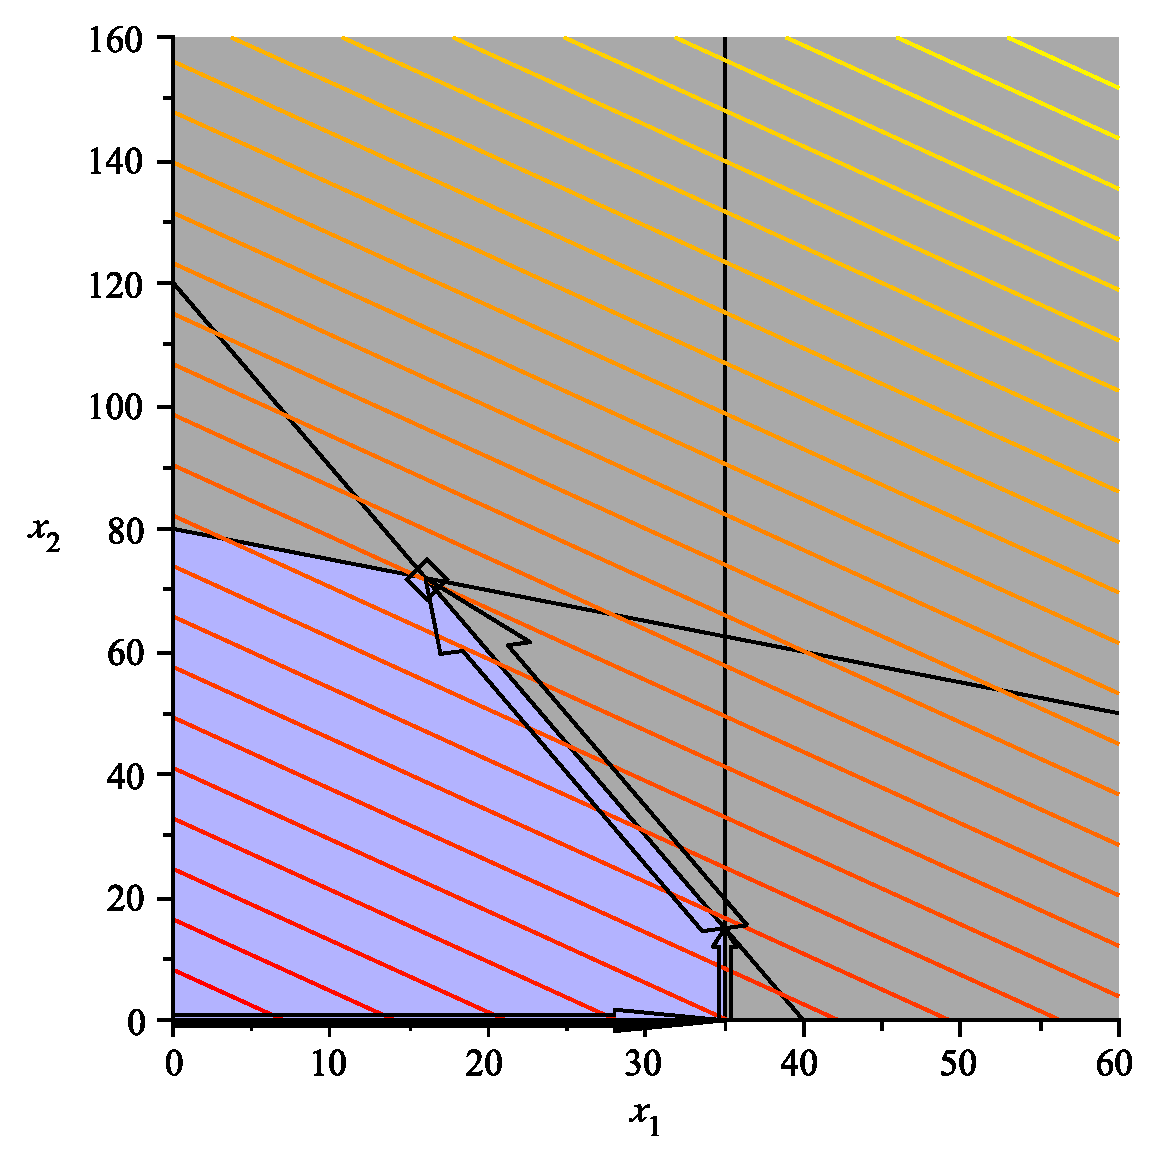
\includegraphics[scale=0.35]{SimplexPath.pdf}
\caption{The Simplex Algorithm: The path around the feasible region is shown in the figure. Each exchange of a basic and non-basic variable moves us along an edge of the polygon in a direction that increases the value of the objective function.}
\label{fig:SimplexPath}
\end{figure}
\label{ex:ToyMakerSimplex}
\end{example}

\begin{exercise} Assume that a leather company manufactures two types of belts: regular and deluxe. Each belt requires 1 square yard of leather. A regular belt requires 1 hour of skilled labor to produce, while a deluxe belt requires 2 hours of labor. The leather company receives 40 square yards of leather each week and a total of 60 hours of skilled labor is available. Each regular belt nets \$3 in profit, while each deluxe belt nets \$5 in profit. The company wishes to maximize profit. 
\begin{enumerate*}
\item Ignoring the divisibility issues, construct a linear programming problem whose solution will determine the number of each type of belt the company should produce. 

\item Use the simplex algorithm to solve the problem you stated above remembering to convert the problem to \textit{standard form} before you begin. 

\item Draw the feasible region and the level curves of the objective function. Verify that the optimal solution you obtained through the simplex method is the point at which the level curves no longer intersect the feasible region in the direction following the gradient of the objective function.
\end{enumerate*}
\label{exer:Leather}
\end{exercise}

\section{Simplex Method--Tableau Form}
No one executes the simplex algorithm in algebraic form. Instead, several representations (tableau representations) have been developed to lesson the amount of writing that needs to be done and to collect all pertinent information into a single table. 

To see how a \textit{Simplex Tableau} is derived, consider Problem $P$ in standard form:
\begin{displaymath}P\left\{
\begin{aligned}
\max\;\;&\mathbf{c}^T\mathbf{x}\\
s.t.\;\;&\mathbf{A}\mathbf{x} = \mathbf{b}\\
& \mathbf{x} \geq \mathbf{0}
\end{aligned}\right.
\end{displaymath}
We can re-write $P$ in an unusual way by introducing a new variable $z$ and separating $\mathbf{A}$ into its basic and non-basic parts to obtain:
\begin{equation}
\begin{aligned}
\max\;\;&z\\
s.t.\;\; &z - \mathbf{c}_\mathbf{B}^T\mathbf{x_B} - \mathbf{c}_\mathbf{N}^T\mathbf{x_N} = 0\\ 
&\mathbf{B}\mathbf{x_B} + \mathbf{N}\mathbf{x_N} = \mathbf{b}\\
& \mathbf{x_B},\mathbf{x_N} \geq 0
\end{aligned}
\end{equation}
From the second equation, it's clear 
\begin{equation}
\mathbf{x_B} + \mathbf{B}^{-1}\mathbf{N}\mathbf{x_N} = \mathbf{B}^{-1}\mathbf{b}
\label{eqn:Row2}
\end{equation}

We can multiply this equation by $\mathbf{c_B^T}$ to obtain:
\begin{equation}
\mathbf{c}_\mathbf{B}^T\mathbf{x_B} + \mathbf{c}_\mathbf{B}^T\mathbf{B}^{-1}\mathbf{N}\mathbf{x_N} = \mathbf{c}_\mathbf{B}^T\mathbf{B}^{-1}\mathbf{b}
\end{equation}
If we add this equation to the equation $z - \mathbf{c}_\mathbf{B}^T\mathbf{x_B} - \mathbf{c}_\mathbf{N}^T\mathbf{x_N} = 0$ we obtain:
\begin{equation}
z + \mathbf{0}^T\mathbf{x_B} + \mathbf{c}_\mathbf{B}^T\mathbf{B}^{-1}\mathbf{N}\mathbf{x_N} - \mathbf{c}_\mathbf{N}^T\mathbf{x_N} = \mathbf{c}_\mathbf{B}^T\mathbf{B}^{-1}\mathbf{b}
\end{equation}
Here $\mathbf{0}$ is the vector of zeros of appropriate size. This equation can be written as:
\begin{equation}
z + \mathbf{0}^T\mathbf{x_B} + \left(\mathbf{c}_\mathbf{B}^T\mathbf{B}^{-1}\mathbf{N} - \mathbf{c}_\mathbf{N}^T\right)\mathbf{x_N} = \mathbf{c}_\mathbf{B}^T\mathbf{B}^{-1}\mathbf{b}
\label{eqn:Row1}
\end{equation}
We can now represent this set of equations as a large matrix (or tableau):
\begin{center}
\begin{tabular}{|c|c|c|c|c|l|}
\hline
& $z$ & $\mathbf{x_B}$ & $\mathbf{x_N}$ & RHS & \\
\hline
$z$ & $1$ & $\mathbf{0}$ & $\mathbf{c}_\mathbf{B}^T\mathbf{B}^{-1}\mathbf{N} - \mathbf{c}_\mathbf{N}^T$ & $\mathbf{c}_\mathbf{B}^T\mathbf{B}^{-1}\mathbf{b}$ & Row 0\\
\hline
$\mathbf{x_B}$ & $\mathbf{0}$ & $\mathbf{1}$ & $\mathbf{B}^{-1}\mathbf{N}$ & $\mathbf{B}^{-1}\mathbf{b}$ & Rows $1$ through $m$\\
\hline
\end{tabular}
\end{center}
The augmented matrix shown within the table:
\begin{equation}
\left[
\begin{array}{ccc|c}
1 & \mathbf{0} & \mathbf{c}_\mathbf{B}^T\mathbf{B}^{-1}\mathbf{N} - \mathbf{c}_\mathbf{N}^T  & \mathbf{c}_\mathbf{B}^T\mathbf{B}^{-1}\mathbf{b}\\
\mathbf{0} & \mathbf{1} & \mathbf{B}^{-1}\mathbf{N} & \mathbf{B}^{-1}\mathbf{b}
\end{array}\right]
\end{equation}
is simply the matrix representation of the simultaneous equations described by Equations \ref{eqn:Row2} and \ref{eqn:Row1}. We can see that the first row consists of a row of the first row of the $(m+1) \times (m+1)$ identity matrix, the reduced costs of the non-basic variables and the current objective function values. The remainder of the rows consist of the rest of the $(m +1) \times (m+1)$ identity matrix, the matrix $\mathbf{B}^{-1}\mathbf{N}$ and $\mathbf{B}^{-1}\mathbf{b}$ the current non-zero part of the basic feasible solution. 

This matrix representation (or tableau representation) contains all of the information we need to execute the simplex algorithm. An entering variable is chosen from among the columns containing the reduced costs and matrix $\mathbf{B}^{-1}\mathbf{N}$. Naturally, a column with a negative reduced cost is chosen. We then chose a leaving variable by performing the minimum ratio test on the chosen column and the right-hand-side (RHS) column. We pivot on the element at the entering column and leaving row and this transforms the tableau into a new tableau that represents the new basic feasible solution.

\begin{example} Again, consider the toy maker problem. We will execute the simplex algorithm using the tableau method. Our problem in standard form is given as:
\begin{displaymath}
\left\{
\begin{aligned}
\max\;\; z(x_1,x_2) = 7x_1 + 6x_2\\
s.t.\;\; 3x_1 + x_2 + s_1 = 120\\
 x_1 + 2x_2 + s_2 = 160\\
 x_1 + s_3 = 35\\
 x_1,x_2,s_1,s_2,s_3\geq 0
\end{aligned}
\right.
\end{displaymath}
We can assume our initial basic feasible solution has $s_1$, $s_2$ and $s_3$ as basic variables and $x_1$ and $x_2$ as non-basic variables. Thus our initial tableau is simply:
\begin{equation}
\begin{array}{c}
\\
z\\
s_1\\
s_2\\
s_3
\end{array}
\left[
\begin{array}{c|ccccc|c}
z& x_1 & x_2 & s_1 & s_2 & s_3 & \text{RHS}\\
\hline
1 & -7 & -6 & 0 & 0 & 0 & 0\\
\hline
0 &  3 &  1 & 1 & 0 & 0 & 120\\
0 &  1 &  2 & 0 & 1 & 0 & 160\\
0 &  1 &  0 & 0 & 0 & 1 & 35\\
\end{array}\right]
\end{equation}
Note that the columns have been swapped so that the identity matrix is divided and $\mathbf{B}^{-1}\mathbf{N}$ is located in columns 2 and 3. This is because of our choice of basic variables. The reduced cost vector is in Row 0.

Using this information, we can see that either $x_1$ or $x_2$ can enter. We can compute the minimum ratio test (MRT) next to the RHS column. If we chose $x_2$ as the entering variable, then the MRT tells us $s_2$ will leave. We put a box around the element on which we will pivot:
\begin{equation}
\begin{array}{c}
\\
z\\
s_1\\
s_2\\
s_3
\end{array}
\left[
\begin{array}{c|ccccc|c}
z& x_1 & x_2 & s_1 & s_2 & s_3 & \text{RHS}\\
\hline
1 & -7 & -6 & 0 & 0 & 0 & 0\\
\hline
0 &  3 &  1 & 1 & 0 & 0 & 120\\
0 &  1 &  \fbox{2} & 0 & 1 & 0 & 160\\
0 &  1 &  0 & 0 & 0 & 1 & 35\\
\end{array}\right]
\begin{array}{c}
\text{MRT ($x_2$)}\\
\hline
\\
120\\
80\\
-
\end{array}
\end{equation}
If we pivot on this element, then we transform the column corresponding to $x_2$ into the identity column:
\begin{equation}
\begin{bmatrix}0 \\ 0 \\ 1 \\ 0
\end{bmatrix}
\end{equation}
This process will correctly compute the new reduced costs and $\mathbf{B}^{-1}$ matrix as well as the new cost information. The new tableau becomes:
\begin{equation}
\begin{array}{c}
\\
z\\
s_1\\
x_2\\
s_3
\end{array}
\left[
\begin{array}{c|ccccc|c}
z& x_1 & x_2 & s_1 & s_2 & s_3 & \text{RHS}\\
\hline
1 & -4 & 0 & 0 & 3 & 0 & 480\\
\hline
0 &  2.5 &  0 & 1 & -0.5 & 0 & 40\\
0 &  0.5 &  1 & 0 & 0.5 & 0 & 80\\
0 &  1 &  0 & 0 & 0 & 1 & 35\\
\end{array}\right]
\end{equation}
We can see that $x_1$ is a valid entering variable, as it has a negative reduced cost ($-4$). We can again place the minimum ratio test values on the right-hand-side of the matrix to obtain:
\begin{equation}
\begin{array}{c}
\\
z\\
s_1\\
x_2\\
s_3
\end{array}
\left[
\begin{array}{c|ccccc|c}
z& x_1 & x_2 & s_1 & s_2 & s_3 & \text{RHS}\\
\hline
1 & -4 & 0 & 0 & 3 & 0 & 480\\
\hline
0 &  \fbox{2.5} &  0 & 1 & -0.5 & 0 & 40\\
0 &  0.5 &  1 & 0 & 0.5 & 0 & 80\\
0 &  1 &  0 & 0 & 0 & 1 & 35\\
\end{array}\right]
\begin{array}{c}
\text{MRT ($x_1$)}\\
\hline
\\
16\\
160\\
35
\end{array}
\end{equation}
We now pivot on the element we have boxed to obtain the new tableau\footnote{Thanks to Ethan Wright for catching a typo here.}:
\begin{equation}
\begin{array}{c}
\\
z\\
x_1\\
x_2\\
s_3
\end{array}
\left[
\begin{array}{c|ccccc|c}
z& x_1 & x_2 & s_1 & s_2 & s_3 & \text{RHS}\\
\hline
1 & 0 & 0 & 1.6 & 2.2 & 0 & 544\\
\hline
0 &  1 &  0 & 0.4 & -0.2 & 0 & 16\\
0 &  0 &  1 & -0.2 & 0.6 & 0 & 72\\
0 &  0 &  0 & -0.4 & 0.2 & 1 & 19\\
\end{array}\right]
\end{equation}
All the reduced costs of the non-basic variables ($s_1$ and $s_2$) are positive and so this is the optimal solution to the linear programming problem. We can also see that this solution agrees with our previous computations on the Toy Maker Problem.
\end{example}

\section{Identifying Unboundedness}
We have already identified a theorem for detecting unboundedness. Recall Theorem \ref{thm:Unboundedness}:
\textit{In a maximization problem, if $\overline{a}_{j_i} < 0$ for all $i = 1,\dots,m$, and $z_j - c_j < 0$, then the linear programming problem is unbounded.}

This condition occurs when a variable $x_j$ should enter the basis because $\partial{z}/\partial{x_j} > 0$ and there is no blocking basis variable. That is, we can arbitrarily increase the value of $x_j$ without causing any variable to become negative. We give an example:
\begin{example} Consider the Linear programming problem from Example \ref{ex:LPUnboundFeasibleRegion1}:
\begin{displaymath}
\left\{
\begin{aligned}
\max\;\;& z(x_1,x_2) = 2x_1 - x_2\\
s.t.\;\;& x_1 - x_2 \leq 1\\
& 2x_1 + x_2 \geq 6\\
&x_1,x_2 \geq 0
\end{aligned}
\right.
\end{displaymath}
We can convert this problem into standard form by adding a slack variable $s_1$ and a surplus variable $s_2$:
\begin{displaymath}
\left\{
\begin{aligned}
\max\;\;& z(x_1,x_2) = 2x_1 - x_2\\
s.t.\;\;& x_1 - x_2 + s_1 = 1\\
& 2x_1 + x_2 - s_2 = 6\\
&x_1,x_2,s_1,s_2 \geq 0
\end{aligned}
\right.
\end{displaymath}

This yields the matrices:
\begin{displaymath}
\mathbf{c} = \begin{bmatrix}2 \\ -1 \\ 0 \\ 0\end{bmatrix}\;\;
\mathbf{x} = \begin{bmatrix}x_1 \\ x_2 \\ s_1 \\ s_2\end{bmatrix}\;\;
\mathbf{A} = \begin{bmatrix} 
1 & -1 & 1 & 0\\
2 & 1 & 0 & -1
\end{bmatrix}\;\;
\mathbf{b} = \begin{bmatrix}1 \\ 6\end{bmatrix}
\end{displaymath}
We have both slack and surplus variables, so the case when $x_1 = x_2 = 0$ is not a valid initial solution. We can chose a valid solution based on our knowledge of the problem. Assume that $s_1 = s_2 = 0$ and so we have:
\begin{displaymath}
\mathbf{B} = \begin{bmatrix}
1 & -1\\
2 & 1
\end{bmatrix}\;\;
\mathbf{N} = \begin{bmatrix}
1 & 0\\
0 & -1
\end{bmatrix}
\end{displaymath}
In this case we have:
\begin{displaymath}
\mathbf{x_B} = \begin{bmatrix}x_1 \\ x_2\end{bmatrix}\;\;
\mathbf{x_N} = \begin{bmatrix}s_1 \\ s_2\end{bmatrix}\;\;
\mathbf{c_B} = \begin{bmatrix}2 \\ -1\end{bmatrix}\;\;
\mathbf{c_N} = \begin{bmatrix}0 \\ 0\end{bmatrix}\;\;
\end{displaymath}
This yields:
\begin{displaymath}
\mathbf{B}^{-1}\mathbf{b} = \begin{bmatrix}7/3 \\ 4/3\end{bmatrix}\;\;
\mathbf{B}^{-1}\mathbf{N} = \begin{bmatrix}1/3 & -1/3 \\ -2/3 & -1/3\end{bmatrix}\;\;
\end{displaymath}
We also have the cost information:
\begin{displaymath}
\mathbf{c_B}\mathbf{B}^{-1}\mathbf{b} = \frac{10}{3}\;\;
\mathbf{c_B}\mathbf{B}^{-1}\mathbf{N} = \begin{bmatrix}\frac{4}{3} & -\frac{1}{3}
\end{bmatrix}\;\;
\mathbf{c_B}\mathbf{B}^{-1}\mathbf{N}-\mathbf{c_N} = \begin{bmatrix}\frac{4}{3} & -\frac{1}{3}
\end{bmatrix}\;\;
\end{displaymath}
Based on this information, we can construct the tableau for this problem as:
\begin{equation}
\begin{array}{c}
\\
z\\
x_1\\
x_2
\end{array}
\left[
\begin{array}{c|cccc|c}
z& x_1 & x_2 & s_1 & s_2 & \text{RHS}\\
\hline
1 &  0 &  0 & \frac{4}{3} & \frac{-1}{3} & \frac{10}{3}\\
\hline
0 &  1 &  0 & \frac{1}{3} & \frac{-1}{3} & \frac{7}{3}\\
0 &  0 &  1 & \frac{-2}{3} & \frac{-1}{3} & \frac{4}{3}
\end{array}\right]
\end{equation}

We see that $s_2$ should enter the basis because $\mathbf{c_B}\mathbf{B}^{-1}\mathbf{A}_{\cdot 4}-\mathbf{c}_4 < 0$. But the column corresponding to $s_2$ in the tabluau is all negative. Therefore there is no minimum ratio test. We can let $s_2$ become as large as we like and we will keep increasing the objective function without violating feasibility. 

What we have shown is that the ray with vertex
\begin{displaymath}
\mathbf{x}_0 = \begin{bmatrix}
7/3\\
4/3\\
0\\
0
\end{bmatrix}
\end{displaymath}
and direction:
\begin{displaymath}
\mathbf{d} = \begin{bmatrix}
1/3\\
1/3\\
0\\
1
\end{bmatrix}
\end{displaymath}
is entirely contained inside the polyhedral set defined by $\mathbf{A}\mathbf{x} = \mathbf{b}$. This can be see from the fact that:
\begin{displaymath}
\mathbf{x_B} = \mathbf{B}^{-1}\mathbf{b} - \mathbf{B}^{-1}\mathbf{N}\mathbf{x_N}
\end{displaymath}
When applied in this case, we have:
\begin{displaymath}
\mathbf{x_B} = \mathbf{B}^{-1}\mathbf{b} - \mathbf{B}^{-1}\mathbf{A}_{\cdot 4}s_2
\end{displaymath}
We know that
\begin{displaymath}
-\mathbf{B}^{-1}\mathbf{A}_{\cdot 4} = 
\begin{bmatrix}
1/3\\
1/3
\end{bmatrix}
\end{displaymath}
We will be increasing $s_2$ (which acts like $\lambda$ in the definition of ray) and leaving $s_1$ equal to $0$. It's now easy to see that the ray we described is contained entirely in the feasible region. This is illustrated in the original constraints in Figure \ref{fig:UnboundedFeasibleRegionSimplex}.
\begin{figure}[htbp]
\centering
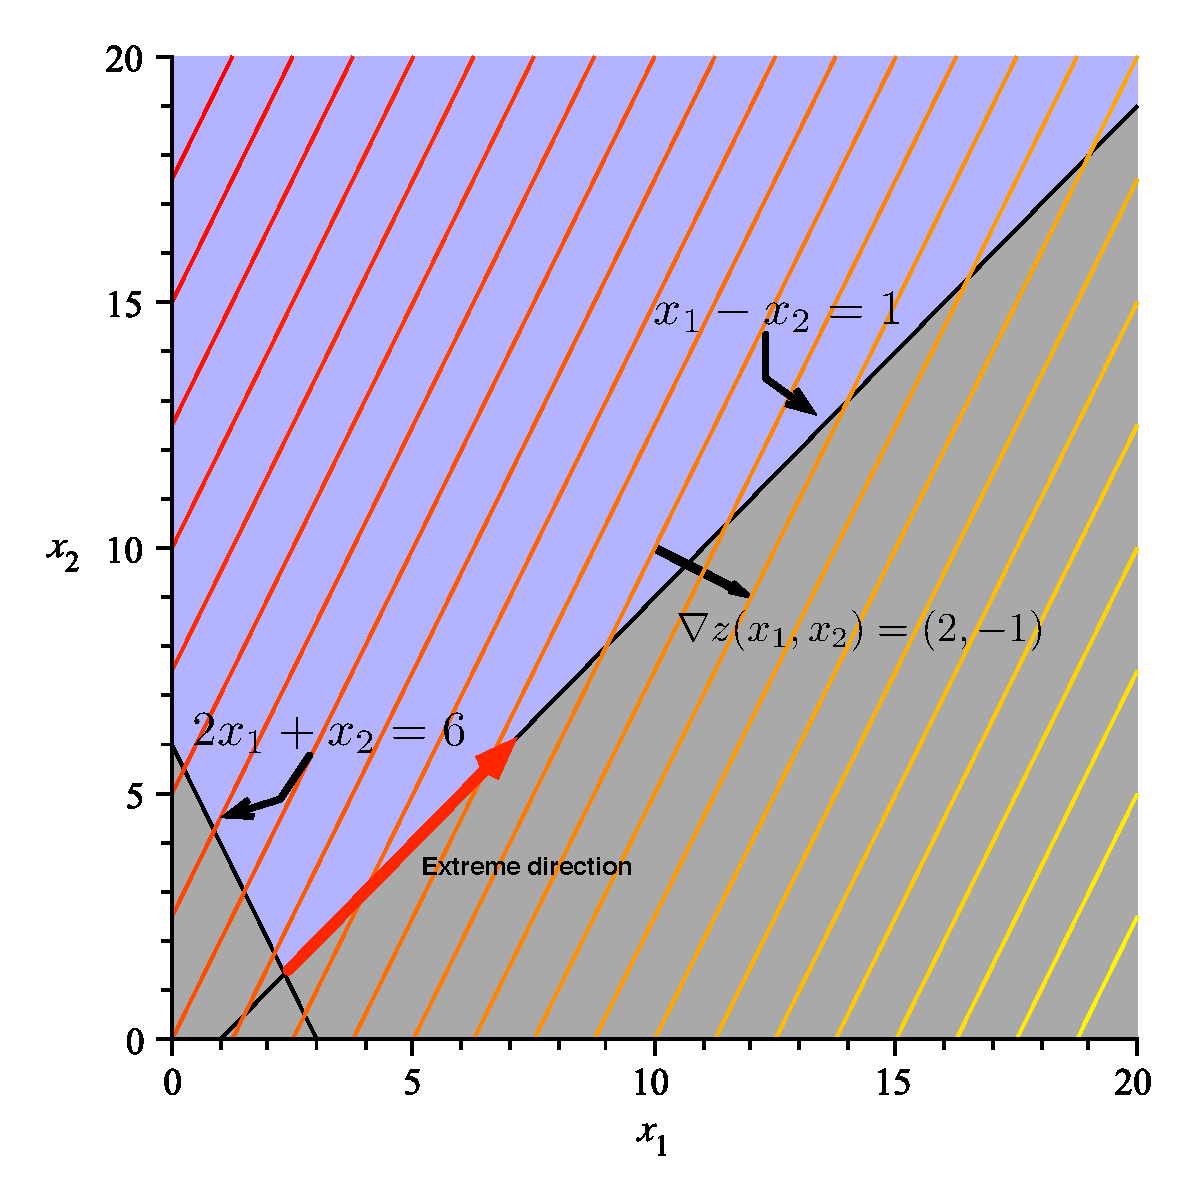
\includegraphics[scale=0.35]{UnboundedFeasibleRegionSimplex.pdf}
\caption{Unbounded Linear Program: The existence of a negative column $\overline{\mathbf{a}}_j$ in the simplex tableau for entering variable $x_j$ indicates an unbounded problem and feasible region. The recession direction is shown in the figure.}
\label{fig:UnboundedFeasibleRegionSimplex}
\end{figure}
\label{ex:UnboundedSolnSimplex}
\end{example}

Based on our previous example, we have the following theorem that extends Theorem \ref{thm:Unboundedness}:
\begin{theorem} In a maximization problem, if $\overline{a}_{j_i} \leq 0$ for all $i = 1,\dots,m$, and $z_j - c_j < 0$, then the linear programming problem is unbounded furthermore, let $\overline{\mathbf{a}}_j$ be the $j^{\text{th}}$ column of $\mathbf{B}^{-1}\mathbf{A}_{\cdot j}$ and let $\mathbf{e}_k$ be a standard basis column vector in $\mathbb{R}^{m \times (n-m)}$ where $k$ corresponds to the position of $j$ in the matrix $\mathbf{N}$. Then the direction:
\begin{equation}
\mathbf{d} = \begin{bmatrix}
-\overline{\mathbf{a}}_j\\
\mathbf{e}_k
\end{bmatrix}
\end{equation}
is an extreme direction of the feasible region $X = \{\mathbf{x} \in \mathbb{R}^n : \mathbf{A}\mathbf{x} = \mathbf{b},\;\mathbf{x} \geq \mathbf{0}\}$.
\label{thm:ExtremeDirectionSimplex} 
\end{theorem}
\begin{proof} The fact that $\mathbf{d}$ is a direction is easily verified by the fact there is an extreme point $\mathbf{x} = [\mathbf{x_B} \; \mathbf{x_N}]^T$ and for all $\lambda \geq 0$ we have:
\begin{equation}
\mathbf{x} + \lambda \mathbf{d} \in X
\end{equation}
Thus it follows from the proof of Theorem \ref{thm:DirectionChar} that $\mathbf{A}\mathbf{d} \leq \mathbf{0}$. The fact that $\mathbf{d} \geq 0$ and $\mathbf{d} \neq 0$ follows from our assumptions. Now, we know that we can write $\mathbf{A} = [\mathbf{B} | \mathbf{N}]$. Further, we know that  $\overline{\mathbf{a}}_j = \mathbf{B}^{-1}\mathbf{A}_{\cdot j}$. Let us consider $\mathbf{A}\mathbf{d}$:
\begin{equation}
\mathbf{A}\mathbf{d} = [\mathbf{B} | \mathbf{N}]\begin{bmatrix}
-\overline{\mathbf{a}}_j\\
\mathbf{e}_k
\end{bmatrix} = 
-\mathbf{B}\mathbf{B}^{-1}\mathbf{A}_{\cdot j} + \mathbf{N}\mathbf{e}_k
\end{equation}
Remember, $\mathbf{e}_k$ is the standard basis vector that has have $1$ precisely in the position corresponding to column $\mathbf{A}_{\cdot j}$ in matrix $\mathbf{N}$, so $\mathbf{A}_{\cdot j} = \mathbf{N} \mathbf{e}_j$. Thus we have:
\begin{equation}
-\mathbf{B}\mathbf{B}^{-1}\mathbf{A}_{\cdot j} + \mathbf{N}\mathbf{e}_k = 
-\mathbf{A}_{\cdot j} + \mathbf{A}_{\cdot j} = \mathbf{0}
\end{equation}
Thus, $\mathbf{A}\mathbf{d} = \mathbf{0}$. We can scale $\mathbf{d}$ so that $\mathbf{e}^T\mathbf{d} = 1$. We know that $n-m-1$ elements of $\mathbf{d}$ are zero (because of $\mathbf{e}_k$) and we know that $\mathbf{A}\mathbf{d} = \mathbf{0}$. Thus $\mathbf{d}$ can be made to represent the intersection of $n$-hyperplanes in $\mathbb{R}^n$. Thus, $\mathbf{d}$ is an extreme point of the polyhedron $D = \{\mathbf{d} \in \mathbb{R}^n : \mathbf{A}\mathbf{d} \leq \mathbf{0}, \mathbf{d}\geq \mathbf{0},\mathbf{e}^T\mathbf{d} = 1\}$. It follows from Theorem \ref{thm:ExtremeDirections}, we know that $\mathbf{d}$ is an extreme direction of $X$. 
\end{proof}

\begin{exercise} Consider the problem 
\begin{displaymath}
\left\{
\begin{aligned}
\min\;\;& z(x_1,x_2) = 2x_1 - x_2\\
s.t.\;\;& x_1 - x_2 + s_1 = 1\\
& 2x_1 + x_2 - s_2 = 6\\
&x_1,x_2,s_1,s_2 \geq 0
\end{aligned}
\right.
\end{displaymath}
Using the rule you developed in Exercise \ref{exer:MinEnteringVariable}, show that the minimization problem has an unbounded feasible solution. Find an extreme direction for this set.
[Hint: The minimum ratio test is the same for a minimization problem. Execute the simplex algorithm as we did in Example \ref{ex:UnboundedSolnSimplex} and use Theorem \ref{thm:ExtremeDirectionSimplex} to find the extreme direction of the feasible region.]
\label{exer:UnboundedMin}
\end{exercise}

\section{Identifying Alternative Optimal Solutions}
We saw in Theorem \ref{thm:SimplixOptimality} that is $z_j - c_j > 0$ for all $j \in \mathcal{J}$ (the indices of the non-basic variables), then the basic feasible solution generated by the current basis was optimal. Suppose that $z_j - c_j \geq 0$. Then we have a slightly different result:
\begin{theorem} In Problem $P$ for a given set of non-basic variables $\mathcal{J}$, if $z_j - c_j \geq 0$ for all $j \in \mathcal{J}$, then the current basic feasible solution is optimal. Further, if $z_j - c_j = 0$ for at least one $j \in \mathcal{J}$, then there are alternative optimal solutions. Furthermore, let $\overline{\mathbf{a}}_j$ be the $j^{\text{th}}$ column of $\mathbf{B}^{-1}\mathbf{A}_{\cdot j}$. Then the solutions to $P$ are:
\begin{equation} 
\left\{
\begin{aligned}
&\mathbf{x_B} = \mathbf{B}^{-1}\mathbf{b}  
-\overline{\mathbf{a}}_jx_j\\
&x_j \in \left[0,
\min\left\{
\frac{\overline{b}_i}{\overline{a}_{j_i}} : i=1,\dots,m,\;\;
\overline{a}_{j_i}>0
\right\}
\right]\\
&x_r = 0, \forall r\in\mathcal{J},\,r\neq j
\end{aligned}\right.
\label{eqn:AltOptSolnForm}
\end{equation}
\end{theorem}
\begin{proof} It follows from the proof of Theorem \ref{thm:SimplixOptimality} that the solution must be optimal as $\partial z/\partial x_j \leq 0$ for all $j \in \mathcal{J}$ and therefore increasing and $x_j$ will \textit{not} improve the value of the objective function. If there is some $j \in \mathcal{J}$ so that $z_j - c_j = 0$, then $\partial z/\partial x_j = 0$ and we may increase the value of $x_j$ up to some point specified by the minimum ratio test, while keeping other non-basic variables at zero. In this case, we will neither increase nor decrease the objective function value. Since that objective function value is optimal, it follows that the set of all such values (described in Equation \ref{eqn:AltOptSolnForm}) are alternative optimal solutions.
\end{proof}
\begin{example}
Let us consider the toy maker problem again from Example \ref{ex:ToyMaker} and \ref{ex:ToyMakerSimplex} with our adjusted objective 
\begin{equation}
z(x_1,x_2) = 18x_1 + 6x_2
\end{equation}
Now consider the penultimate basis from Example \ref{ex:ToyMakerSimplex} in which we had as basis variables $x_1$, $s_2$ and $x_2$. 
\begin{displaymath}
\mathbf{x_B} = \begin{bmatrix}x_1\\x_2\\s_2\end{bmatrix}\;\;
\mathbf{x_N} = \begin{bmatrix}s_1\\s_3\end{bmatrix}\;\;
\mathbf{c_B} = \begin{bmatrix}18\\6\\0\end{bmatrix}\;\;
\mathbf{c_N} = \begin{bmatrix}0\\0\end{bmatrix}
\end{displaymath}
The matrices become:
\begin{displaymath}
\mathbf{B} = \begin{bmatrix}
3 & 1 & 0\\
1 & 2 & 1\\
1 & 0 & 0
\end{bmatrix}\;\;
\mathbf{N} = \begin{bmatrix}
1 & 0\\
0 & 0\\
0 & 1
\end{bmatrix}
\end{displaymath}
The derived matrices are then:
\begin{displaymath}
\mathbf{B}^{-1}\mathbf{b} = \begin{bmatrix}35\\15\\95\end{bmatrix}\;\;
\mathbf{B}^{-1}\mathbf{N} = \begin{bmatrix}
0  & 1\\
1  & -3\\
-2 & 5
\end{bmatrix}
\end{displaymath}
The cost information becomes:
\begin{displaymath}
\mathbf{c}_\mathbf{B}^T\mathbf{B}^{-1}\mathbf{b} = 720 \;\;\;
\mathbf{c}_\mathbf{B}^T\mathbf{B}^{-1}\mathbf{N} = \begin{bmatrix}6 & 0\end{bmatrix}\;\;\;
\mathbf{c}_\mathbf{B}^T\mathbf{B}^{-1}\mathbf{N} - \mathbf{c_N} = 
\begin{bmatrix}6 & 0\end{bmatrix}
\end{displaymath}
This yields the tableau:
\begin{equation}
\begin{array}{c}
\\
z\\
s_1\\
s_2\\
s_3
\end{array}
\left[
\begin{array}{c|ccccc|c}
z& x_1 & x_2 & s_1 & s_2 & s_3 & \text{RHS}\\
\hline
1 &  0 & 0 & 6 & 0 & \textbf{0} & 720\\
\hline
0 &  1 & 0 & 0 & 0 & 1  		 & 35\\
0 &  0 & 1 & 1 & 0 & -3 		 & 15\\
0 &  0 & 0 & -2& 1 & 5 		 	 & 95\\
\end{array}\right]
\end{equation}

Unlike example \ref{ex:ToyMakerSimplex}, the reduced cost for $s_3$ is $0$. This means that if we allow $s_3$ to enter the basis, the objective function value will not change. Performing the minimum ratio test however, we see that $s_2$ will still leave the basis:
\begin{equation}
\begin{array}{c}
\\
z\\
x_1\\
x_2\\
s_2
\end{array}
\left[
\begin{array}{c|ccccc|c}
z& x_1 & x_2 & s_1 & s_2 & s_3 & \text{RHS}\\
\hline
1 &  0 & 0 & 6 & 0 & \textbf{0} & 720\\
\hline
0 &  1 & 0 & 0 & 0 & 1  		 & 35\\
0 &  0 & 1 & 1 & 0 & -3 		 & 15\\
0 &  0 & 0 & -2& 1 & \fbox{5} 		 	 & 95\\
\end{array}\right]
\begin{array}{c}
\text{MRT ($s_3$)}\\
\hline
\\
35\\
-\\
19
\end{array}
\end{equation}


Therefore any solution of the form:
\begin{equation}
\begin{aligned}
&s_3 \in [0,19]\\
&\begin{bmatrix}
x_1\\
x_2\\
s_2
\end{bmatrix} = 
\begin{bmatrix}35\\15\\95\end{bmatrix} - 
\begin{bmatrix}1\\-3\\5\end{bmatrix}s_3
\end{aligned}
\label{eqn:InfAltOptSimplex}
\end{equation}
is an optimal solution to the linear programming problem. This precisely describes the edge shown in Figure \ref{fig:InfiniteOptSoln2}.
\begin{figure}[htbp]
\centering
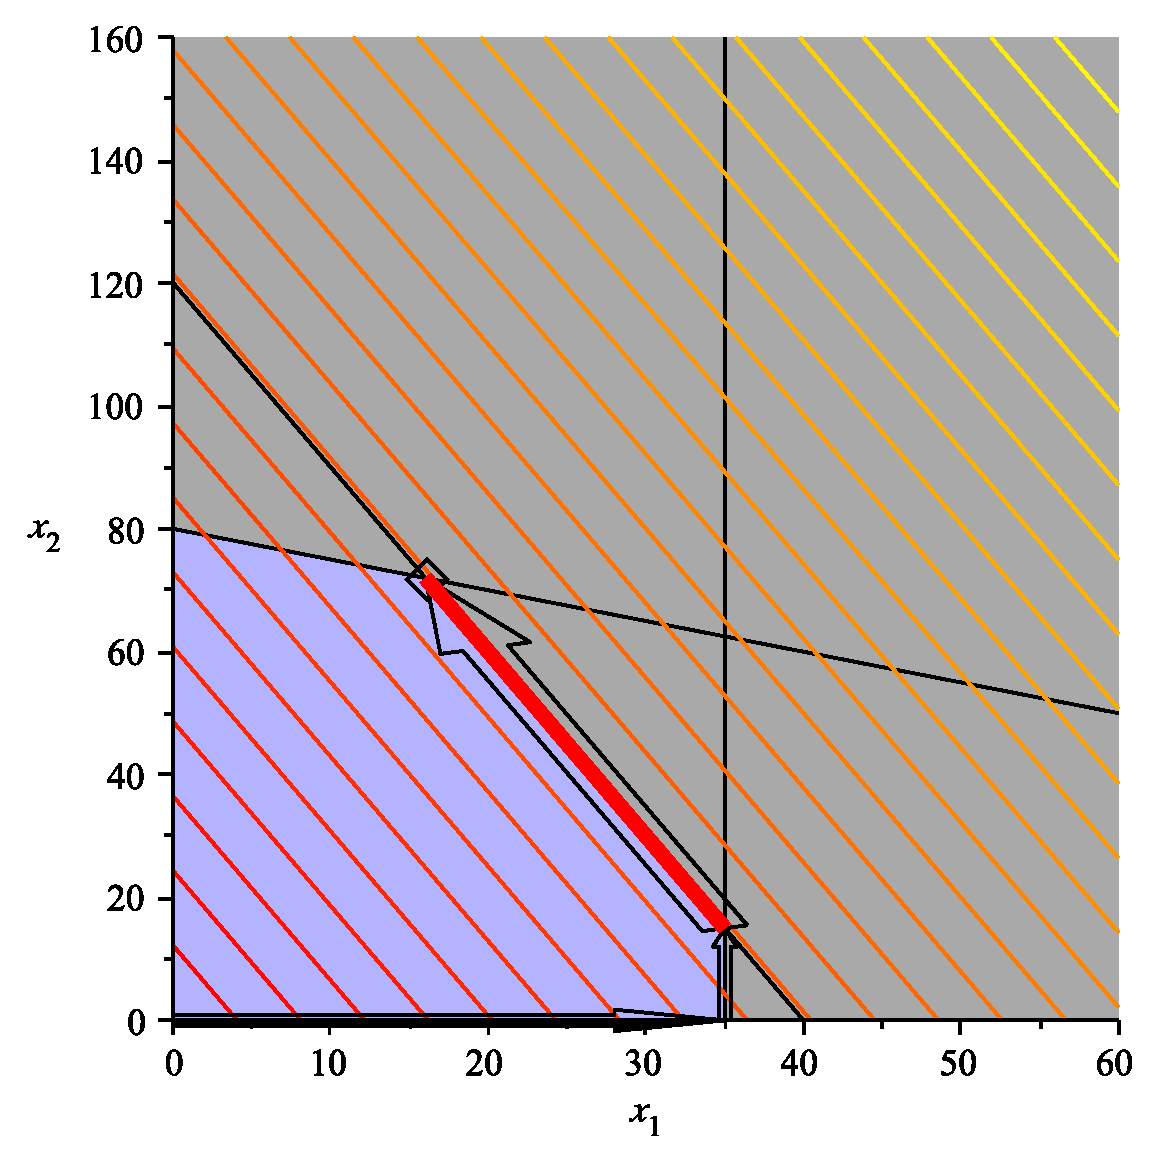
\includegraphics[scale=0.35]{InfOptSimplex.pdf}
\caption{Infinite alternative optimal solutions: In the simplex algorithm, when $z_j - c_j \geq 0$ in a maximization problem with at least one $j$ for which $z_j - c_j = 0$, indicates an infinite set of alternative optimal solutions.}
\label{fig:InfiniteOptSoln2}
\end{figure}
\end{example}

\begin{exercise} Consider the diet problem we covered in Example \ref{ex:Diet}. I wish to design a diet consisting of Raman noodles and ice cream. I'm interested in spending as little money as possible but I want to ensure that I eat at least 1200 calories per day and that I get at least 20 grams of protein per day. Assume that each serving of Raman costs \$1 and contains 100 calories and 2 grams of protein. Assume that each serving of ice cream costs \$1.50 and contains 200 calories and 3 grams of protein. 
\begin{enumerate}
\item Develop a linear programming problem that will help me minimize the cost of my food intake. 
\item Remembering to transform the linear programming problem you found above into standard form, use the simplex algorithm to show that this problem has an infinite set of alternative optimal solutions. 
\item At an optimal extreme point, find an expression for the set of infinite alternative optimal exteme points like the one shown in Equation \ref{eqn:InfAltOptSimplex}. 
\item Plot the feasible region and the level curves of the objective function. Highlight the face of the polyhedral set on which the alternative optimal solutions can be found.
\end{enumerate}

\end{exercise}

\section{Degeneracy and Convergence}
In this section we give an example of degeneracy and its impact on the simplex algorithm. 

\begin{example}
Consider the modified form of the toy maker problem originally stated in Example \ref{ex:ToyMakerDegen}:
\begin{equation}
\left\{
\begin{aligned}
\max\;\;&7x_1 + 6x_2\\
s.t.\;\;&3x_1 + x_2 \leq 120\\
&x_1 + 2x_2 \leq 160\\
&x_1 \leq 35\\
&\frac{7}{4}x_1+x_2 \leq 100\\
&x_1,x_2 \geq 0
\end{aligned}
\right.
\end{equation}
The polyhedral set and level curves of the objective function are shown Figure \ref{fig:DegenOptim}.
\begin{figure}[htbp]
\centering
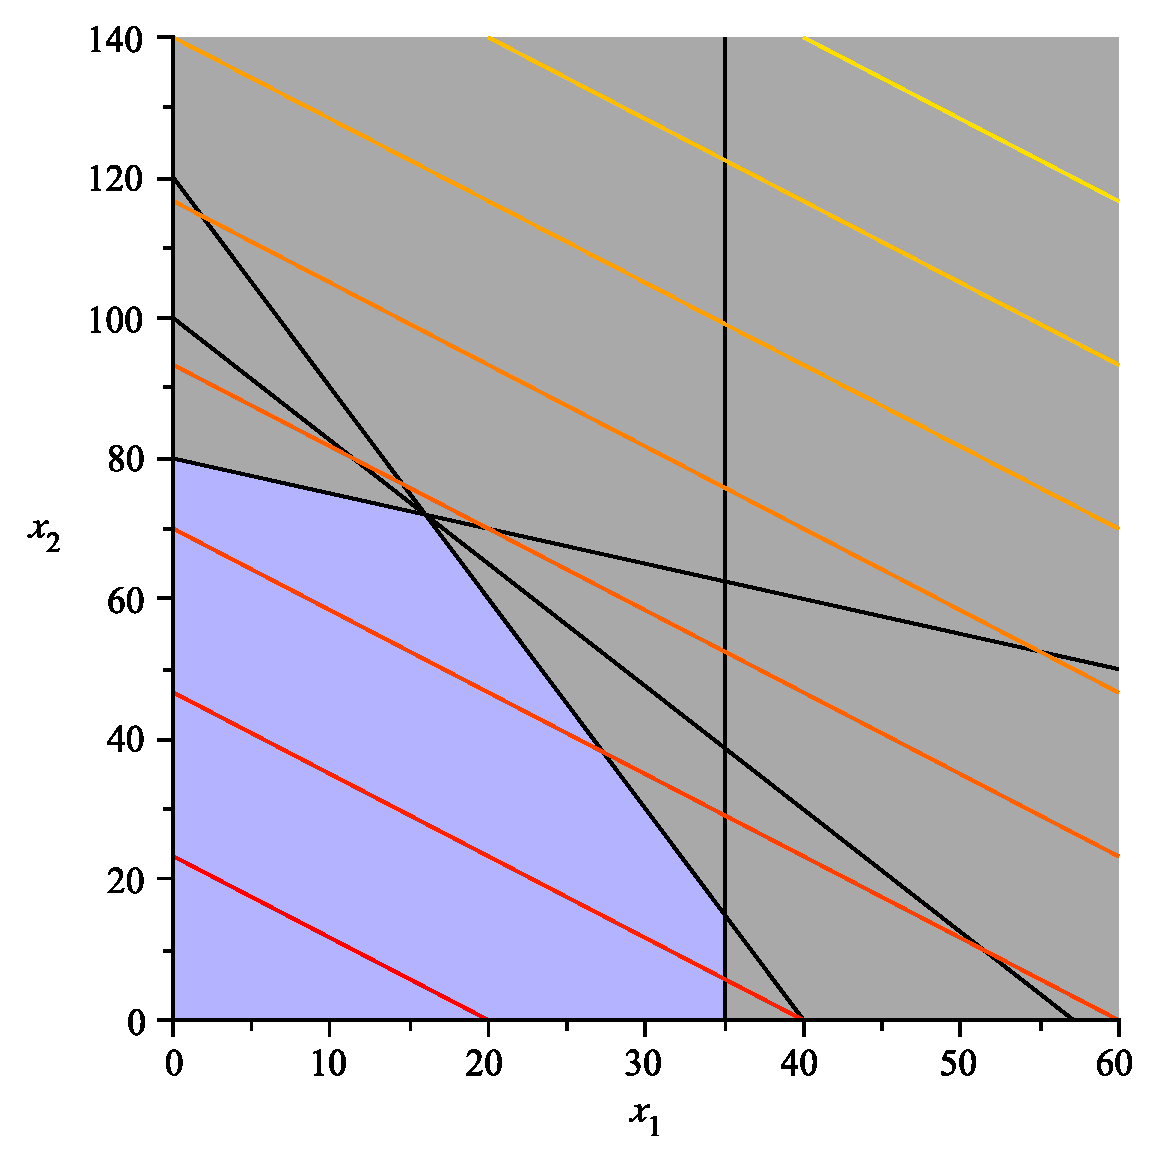
\includegraphics[scale=0.35]{DegenOptim.pdf}
\caption{An optimization problem with a degenerate extreme point: The optimal solution to this problem is still $(16,72)$, but this extreme point is degenerate, which will impact the behavior of the simplex algorithm.}
\label{fig:DegenOptim}
\end{figure}
We can convert the problem to standard form by introducing slack variables:
\begin{equation}
\left\{
\begin{aligned}
\max\;\;&7x_1 + 6x_2\\
s.t.\;\;&3x_1 + x_2 +s_1 = 120\\
&x_1 + 2x_2 + s_2 = 160\\
&x_1 + s_3 = 35\\
&\frac{7}{4}x_1+x_2 + s_4 = 100\\
&x_1,x_2,s_1,s_2,s_3,s_4 \geq 0
\end{aligned}
\right.
\end{equation}

Suppose we start at the extreme point where $x_1 = 35$ and $x_2 = 15$ and $s_2 = 95$ and $s_4 = 23.75$. In this case, the matrices are:
\begin{displaymath}
\mathbf{B} = \begin{bmatrix}
3 & 	1 & 0 & 0\\
1 & 	2 & 1 & 0\\
1 & 	0 & 0 & 0\\
7/4 & 1 & 0 & 1
\end{bmatrix}\;\;
\mathbf{N} = \begin{bmatrix}
1 & 0\\
0 & 0\\
0 & 1\\
0 & 0
\end{bmatrix}
\end{displaymath}
\begin{displaymath}
\mathbf{B}^{-1}\mathbf{b} = \begin{bmatrix}
35\\
15\\
95\\
\frac{95}{4}
\end{bmatrix}\;\;
\mathbf{B}^{-1}\mathbf{N} = \begin{bmatrix}
0 & 1\\
1 & -3\\
-2 & 5\\
-1 & \frac{5}{4}
\end{bmatrix}
\end{displaymath}
\begin{displaymath}
\mathbf{c_B}\mathbf{B}^{-1}\mathbf{b} = 335\;\;
\mathbf{c_B}\mathbf{B}^{-1}\mathbf{N} - \mathbf{c_N} = \begin{bmatrix} 6 & -11\end{bmatrix}
\end{displaymath}
The tableau representation is:
\begin{equation}
\begin{array}{c}
\\
z\\
x_1\\
x_2\\
s_2\\
s_4
\end{array}
\left[
\begin{array}{c|cccccc|c}
z& x_1 & x_2 & s_1 & s_2 & s_3 & s_4 &\text{RHS}\\
\hline
1 & 0 & 0 & 6 & 0 & -11 & 0 & 335\\
\hline
0 & 1 & 0 & 0 & 0 & 1 & 0 & 35\\
0 & 0 & 1 & 1 & 0 & -3 & 0 & 15\\
0 & 0 & 0 & -2 & 1 & 5 & 0 & 95\\
0 & 0 & 0 & -1 & 0 & \fbox{5/4} & 1 & \frac{95}{4}
\end{array}\right]
\begin{array}{c}
\text{MRT ($s_3$)}\\
\hline
\\
35\\
-\\
19\\
19
\end{array}
\end{equation}

From this, we see that the variable $s_3$ should enter (because its reduce cost is negative). In this case, there is a tie for the leaving variables: we see that $95/5 = 19 = (95/4)/(5/4)$, therefore, either $s_2$ or $s_4$ could be chosen as the leaving variable. This is because we will move to a degenerate extreme point when $s_3$ enters the basis. 

Suppose we choose $s_4$ as the leaving variable. Then our tableau will become:
\begin{equation}
\begin{array}{c}
\\
z\\
x_1\\
x_2\\
s_2\\
s_3
\end{array}
\left[
\begin{array}{c|cccccc|c}
z& x_1 & x_2 & s_1 & s_2 & s_3 & s_4 &\text{RHS}\\
\hline
1 & 0 & 0 & -14/5 & 0 & 0 & 44/5 & 544\\
\hline
0 & 1 & 0 & 4/5 			& 0 & 0  & -4/5 & 16\\
0 & 0 & 1 & -7/5 			& 0 & 0  & 12/5 & 72\\
0 & 0 & 0 & \fbox{2} 		& 1 & 0  & -4 	& 0\\
0 & 0 & 0 & -4/5 			& 0 & 1  & 4/5 	& 19
\end{array}\right]
\begin{array}{c}
\text{MRT ($s_1$)}\\
\hline
\\
20\\
-\\
0\\
-
\end{array}
\end{equation}

We now observe two things: 
\begin{enumerate*}
\item One of the basic variables ($s_2$) is zero, even though it is basic. This is \textit{the indicator} of degeneracy at an extreme point. 

\item The reduced cost of $s_1$ is negative, indicating that $s_1$ should enter the basis. 
\end{enumerate*}
If we choose $s_1$ as an entering variable, then using the minimum ratio test, we will choose $s_2$ as the leaving variable (by the minimum ratio test)\footnote{The minimum ratio test still applies when $\overline{\mathbf{b}}_{j} = 0$. In this case, we will remain at the same extreme point.}.   
Then the tableau becomes:
\begin{equation}
\begin{array}{c}
\\
z\\
x_1\\
x_2\\
s_1\\
s_3
\end{array}
\left[
\begin{array}{c|cccccc|c}
z& x_1 & x_2 & s_1 & s_2 & s_3 & s_4 &\text{RHS}\\
\hline
1 & 0 & 0 & 0 & 7/5 	& 0 & 16/5 & 544\\
\hline
0 & 1 & 0 & 0 & -2/5 		& 0  & 4/5 		& 16\\
0 & 0 & 1 & 0 & 7/10 		& 0  & -2/5 	& 72\\
0 & 0 & 0 & 1 & 1/2 		& 0  & -2 		& 0\\
0 & 0 & 0 & 0 & 2/5 		& 1  & -4/5 	& 19
\end{array}\right]
\end{equation}

Notice the objective function value $\mathbf{c_B}\mathbf{B}^{-1}\mathbf{b}$ has \textit{not} changed, because we really have not moved to a new extreme point. We have simply changed from one representation of the degenerate extreme point to another. This was to be expected, the fact that the minimum ratio was zero showed that we could not increase $s_1$ and maintain feasibility. As such $s_1 = 0$ in the new basic feasible solution. The reduced cost vector $\mathbf{c_B}\mathbf{B}^{-1}\mathbf{N} - \mathbf{c_N}$ has changed and we could now terminate the simplex method. 
\label{ex:ToyMakerDegenSimplex}
\end{example}

\begin{theorem} Consider Problem $P$ (our linear programming problem). Let $\mathbf{B} \in \mathbb{R}^{m\times m}$ be a basis matrix corresponding to some set of basic variables $\mathbf{x_B}$. Let $\overline{\mathbf{b}} = \mathbf{B}^{-1}\mathbf{b}$. If $\overline{\mathbf{b}}_j = 0$ for some $j=1,\dots,m$, then $\mathbf{x}_B = \overline{\mathbf{b}}$ and $\mathbf{x_N} = \mathbf{0}$ is a degenerate extreme point of the feasible region of Problem $P$.
\label{thm:DegeneracyDef}
\end{theorem}
\begin{proof} At any basic feasible solutions we have chosen $m$ variables as basic. This basic feasible solution satisfies $\mathbf{B}\mathbf{x_B} = \mathbf{b}$ and thus provides $m$ binding constraints. The remaining variables are chosen as non-basic and set to zero, thus $\mathbf{x_N} = \mathbf{0}$, which provides $n-m$ binding constraints on the non-negativity constraints (i.e., $\mathbf{x} \geq \mathbf{0}$). If there is a basic variable that is zero, then an extra non-negativity constraint is binding at that extreme point. Thus $n+1$ constraints are binding and, by definition, the extreme point must be degenerate. 
\end{proof}

\subsection{The Simplex Algorithm and Convergence}
Using the work we've done in this chapter, we can now state the following implementation of the Simplex algorithm in matrix form. 

\begin{algorithm}
\caption{The Matrix form of the Simplex Algorithm}
\label{alg:SimplexMatrixForm}
\begin{center}
\begin{minipage}[t]{\textwidth-1em}
\underline{\textbf{Simplex Algorithm in Algebraic Form}}
\begin{enumerate*}
\item Given Problem $P$ in \textbf{standard form} with cost vector $\mathbf{c}$, coefficient matrix $\mathbf{A}$ and right hand side $\mathbf{b}$, identify an initial basic feasible solution $\mathbf{x_B}$ and $\mathbf{x_N}$ by any means. Let $\mathcal{J}$ be the set of indices of non-basic variables. If no basic feasible solution can be found, \textbf{STOP}, the problem has no solution.

\item Compute the row vector $\mathbf{c}_\mathbf{B}^T\mathbf{B}^{-1}\mathbf{N} - \mathbf{c}_\mathbf{N}^T$. This vector contains $z_j - c_j$ for $j \in \mathcal{J}$. 

\item If $z_j - c_j \geq 0$ for all $j \in \mathcal{J}$, \textbf{STOP}, the current basic feasible solution is optimal. Otherwise, Goto 4.

\item Choose a non-basic variable $x_j$ with $z_j-c_j < 0$. Select $\overline{\mathbf{a}}_j$ from $\mathbf{B}^{-1}\mathbf{N}$. If $\overline{\mathbf{a}}_j \leq 0$, then the problem is unbounded, \textbf{STOP}. Otherwise Goto 5.

\item Let $\overline{\mathbf{b}} = \mathbf{B}^{-1}\mathbf{b}$. Find the index $i$ solving: 
\begin{displaymath}
\min\left\{
\overline{\mathbf{b}}_i/\overline{\mathbf{a}}_{j_i} : i = 1,\dots,m \text{ and } \overline{\mathbf{a}}_{j_i}\geq 0
\right\}
\end{displaymath}
 
\item Set $\mathbf{x_B}_i = 0$ and $x_j = \overline{\mathbf{b}}_i/\overline{\mathbf{a}}_{j_i}$. 

\item Update $\mathcal{J}$ and GOTO Step 2
\end{enumerate*}
\end{minipage}
\end{center}
\end{algorithm}

\begin{exercise} State the simplex algorithm in Tableau Form. [Hint: Most of the simplex algorithm is the same, simply add in the row-operations executed to compute the new reduced costs and $\mathbf{B}^{-1}\mathbf{N}$.]
\end{exercise}

\begin{theorem} If the feasible region of Problem $P$ has no degenerate extreme points, then the simplex algorithm will terminate in a finite number of steps with an optimal solution to the linear programming problem. 
\label{thm:SimpleConvergence}
\end{theorem}
\begin{proof}[Sketch of Proof] In the absence of degeneracy, the value of the objective function improves (increases in the case of a maximization problem) each time we exchange a basic variable and non-basic variable. This is ensured by the fact that the entering variable always has a negative reduced cost. There are a finite number of extreme points for each polyhedral set, as shown in Lemma \ref{lem:FiniteExtremePoints}. Thus, the process of moving from extreme point to extreme point of $X$, the polyhedral set in Problem $P$ must terminate with the largest possible objective function value. 
\end{proof}

\begin{remark} The correct proof that the simplex algorithm converges to a point of optimality is actually proved by showing that the algorithm terminates with something called a Karush-Kuhn-Tucker (KKT) point. Unfortunately, we will not study the Karush-Kuhn-Tucker conditions until later. There are a few proofs that do not rely on showing that the point of optimality is a KKT point (see \cite{Dan60} for example), but most rely on some intimate knowledge or assumptions on polyhedral sets and are not satisfying. Thus, for students who are not as concerned with the intricate details of the proof, the previous proof sketch is more than sufficient to convince you that the simplex algorithm is correct. For those students who prefer the rigorous detail, please see Chapter \ref{chap:KKT}.
\end{remark}

